%!TEX root = proyecto.tex

\chapter{Estado del arte}

El reconocimiento facial es un ámbito de la visión artificial, que como su nombre indica, se centra en la búsqueda de rostros humanos dentro de imágenes digitales. Durante años se han desarrollado varias tecnologías capaces de realizar dicha acción, de las que se pueden distinguir dos grupos: aplicaciones con y sin el uso de \textit{Deep Learning}. Aunque, ambos se centran en las características de los rostros humanos para lograr identificarlos, conocidas como \textit{features}. Corresponden con puntos de la cara muy reconocibles, como: el mentón, ojos, cejas, nariz, etc. Esta técnica fue usada por primera vez en 2001, por Paul Viola y Michael Jones, y desde entonces se ha convertido en unas de las técnicas principales en el reconocimiento facial.

Este ejercicio se complica cuando las imágenes presentan errores naturales en su toma (como baja luz, ruido, etc.) o los individuos visten complementos que tapen sus rasgos faciales. Este es el problema que se va a plantear en este trabajo, buscar una posible solución al reconocimiento facial con complementos faciales, en especifico identificar si las personas llevan mascarillas.

\section{Python y OpenCV}

Python es un lenguaje de programación \textit{Open Source} y de alto nivel, que permite trabajar y desarrollar aplicaciones de forma rápida y sencilla. Además, se trata de un lenguaje que ha aumentado en popularidad los últimos años gracias a su gran uso en ramas de la tecnología emergente, como \textit{Data Science}, Inteligencia Artificial, \textit{Big Data} o Visión Artificial. En esta última gracias a la existencia de una herramienta llamada \textit{OpenCV}, librería \textit{Open Source} centrada en la creación de aplicaciones en tiempo real sobre visión artificial, que cuenta con una gran cantidad de implementaciones de algoritmos de \textit{Computer Vision}.

\section{Aplicaciones sin Deep Learning}

Entre los años 2000 y 2015 se implementaron varias soluciones para el problema de la identificación facial. Centrados, su mayoría, en la extracción de caracteristicas del rostro humano mediante técnicas de procesamiento de imágenes digitales. Son importante de destacar los siguientes avances durante estos años:

\begin{enumerate}
	\item \textbf{HAAR-like Features \& ADABOOST}.
	
	Técnica diseñada por Paul Viola y Michael Jones en el año 2001, donde se implementa una detección mediante el uso de \textit{Machine Learning} que es capaz de procesar imágenes a una velocidad y precisión bastante altos (Figura \ref{fig:haarExample}), comparado con los desarrollos de la época, gracias al uso de técnicas avanzadas de procesamiento de imágenes y de un modelo de \textit{Machine Learning} llamado \textit{AdaBoost} \cite{paulViola}. 
	
	\begin{figure}[htp]
		\centering
		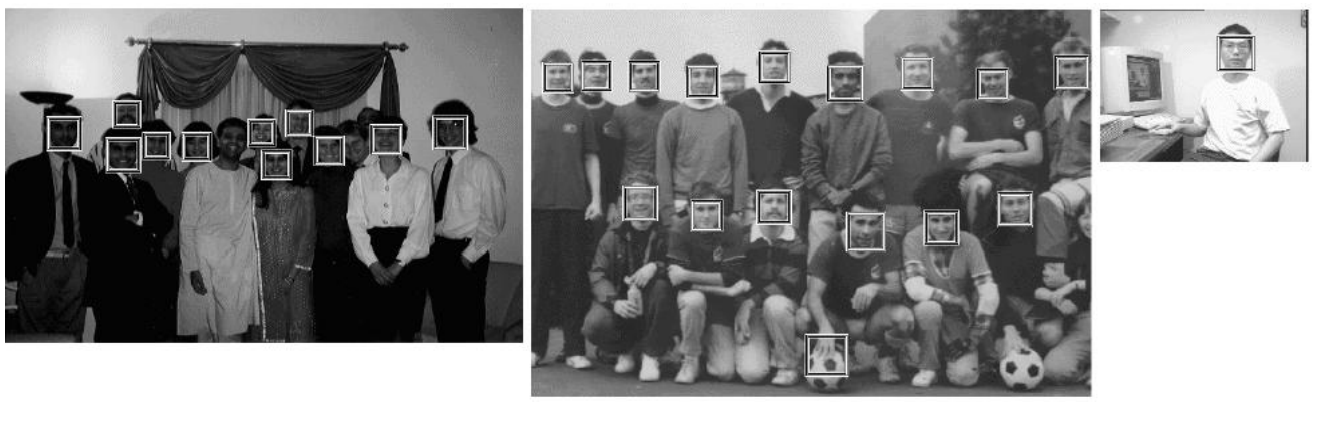
\includegraphics[width=10cm]{imagenes/violayjones_detector.png}
		\caption{Salida generada por el detector facial \cite{paulViola}.}
		\label{fig:haarExample}
	\end{figure}
	
	\item \textbf{HOG} (Histogram of Gradient).
	
	Se trata de una técnica de detección de rostros u otro tipo de objetos mediante el uso de gradientes, término dedicado al estudio de la dirección de un punto en la imagen utilizando derivadas (Figura \ref{fig:hogExample}). Estos servirán para el entrenamiento de un clasificador SVM (\textit{Super Vector Machine}), que será capaz de realizar una detección en tiempo real.
	
	\begin{figure}[htp]
		\centering
		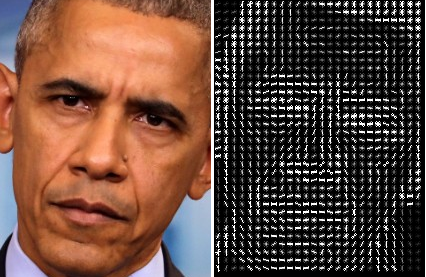
\includegraphics[width=5cm]{imagenes/hog_example.png}
		\caption{HOG generada tras estudiar un rostro.}
		\label{fig:hogExample}
	\end{figure}
	
	\item \textbf{Facial Landmarks}.
	
	Con la aparición de técnicas como las anteriores, se dio el siguiente paso con la predicción de puntos de interés sobre los rostros detectados (Figura \ref{fig:landmarkExample}). El desarrollo de esta se realiza con el uso de técnicas llamadas: \textit{Gradient Boosting} y \textit{Ensemble of regression trees}, ambas del ámbito del \textit{Machine Learning} \cite{faceLandmark}. Cabe destacar, que esta técnica detecta rasgos faciales (como boca, nariz u ojos) aunque se encuentren escondidos tras algún complemento u objeto, gracias al uso de la predicción.
	
	\begin{figure}[htp]
		\centering
		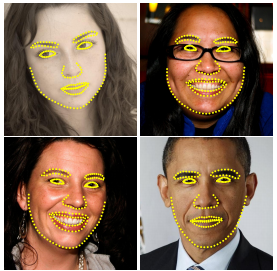
\includegraphics[width=5cm]{imagenes/landmark_example.png}
		\caption{Salidas de ejemplo de Facial Landmark \cite{faceLandmark}.}
		\label{fig:landmarkExample}
	\end{figure}
	
\end{enumerate}


\section{Aplicaciones con Deep Learning}

A partir de 2016, el \textit{Deep Learning} fue un ámbito que gano mucha importancia en la visión artificial. Basado en estructuras CNN (\textit{Convolutional Neural Network}), capaces de extraer las características de las imágenes de entrada mediante el uso de filtros. Algunas de las principales implementaciones del \textit{Deep Learning} para la detección de objetos/rostros son:

\begin{enumerate}
	\item \textbf{YOLO}.
	
	Modelo capaz de procesar imágenes en tiempo real a una velocidad de 45 frames por segundo (con una GPU Nvidia Titan X), con el uso de una única red convolucional (CNN) que predice simultáneamente varios tipos de clases de objetos (Figura \ref{fig:yoloExample}). Este modelo es entrenado mediante imágenes completas \cite{YOLO}.
	
	\begin{figure}[htp]
		\centering
		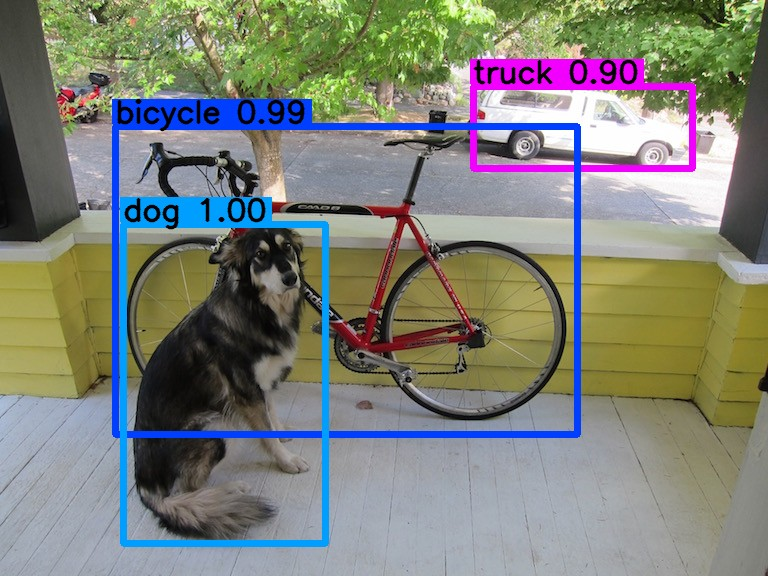
\includegraphics[width=5cm]{imagenes/yolo_example.jpg}
		\caption{Detecciones de ejemplo de YOLO.}
		\label{fig:yoloExample}
	\end{figure}
	
	\item \textbf{TensorFlow}.
	
	TensorFlow es una plataforma de \textit{Open Source} dedicada al aprendizaje automático. Permite compilar e implementar con facilidad aplicaciones con tecnología de AA. En el ámbito de la visión artificial, dispone de una gran cantidad de modelos pre-entrenados capaces de realizar detección de objetos y clasificación de imágenes de forma rápida y precisa. Entre dichos modelos destaca \textit{MobileNet}, capaz de obtener un gran rendimiento en dispositivos móviles y ordenadores con poca potencia computacional (Figura \ref{fig:mobilenetExample}). Esto ha creado un aumento de la popularidad en la implementaciones de detectores en dispositivos embebidos, como \textit{Raspberry Pi}, o en chips ESP32 mediante procesamiento remoto.
	
	\begin{figure}[htp]
		\centering
		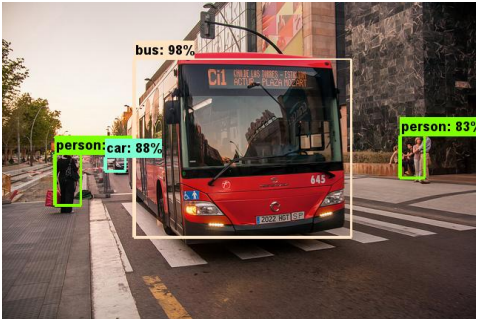
\includegraphics[width=7cm]{imagenes/mobilenet_example.png}
		\caption{Ejemplo de detección con el modelo MobileNet y Tensorflow \cite{mobilenet1}.}
		\label{fig:mobilenetExample}
	\end{figure}
	
	\item \textbf{MediaPipe}.
	
	MediaPipe \cite{mediapipe} es un framework creado por Google centrado en el desarrollo de aplicaciones de visión artificial de forma sencilla y potente. Este se basa en un modelo propio llamado \textit{BlazeFace}, inspirado en modelos como \textit{MobileNet}. Entre sus soluciones (Figura \ref{fig:solMed}) se pueden encontrar: detección facial, predicción de una malla facial (Face Landmarks), detector de iris, detector de manos, reconocer poses, segmentación de pelo, etc.
	
	\begin{figure}[htp]
		\centering
		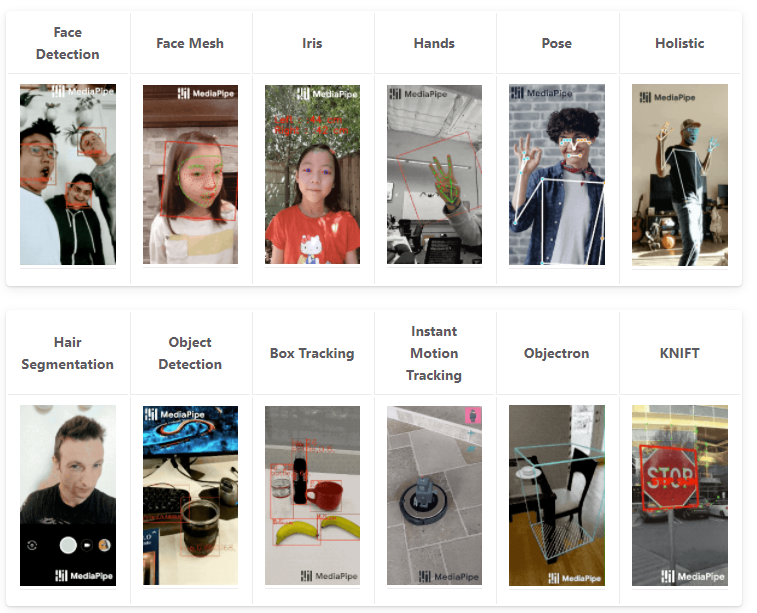
\includegraphics[width=7cm]{imagenes/solucionesMediaPipe.png}
		\caption{Soluciones de MediaPipe \cite{mdSolutions}.}
		\label{fig:solMed}
	\end{figure}
	
	\item \textbf{IBM Watson}.
	
	IBM Watson es un servicio ofrecido por IBM, que permite la creación de aplicaciones de inteligencia artificial en la nube. Este tipo de servicios nos permiten crear aplicaciones potentes sin necesidad de disponer de una gran potencia computacional en nuestra casa. Concretamente, IBM Watson dispone de un módulo llamado \textit{Visual Recognition} que permite el análisis de imágenes y detección de objetos. Este tipo de servicios son de pago, pero permiten una cantidad de procesado gratuita. En este caso, IBM permite tener dos modelos personalizados y 1000 eventos de forma gratuita al mes \cite{ibm}. 
\end{enumerate}



